\documentclass[11pt,twocolumn]{article}
\usepackage[margin=.75in]{geometry}
\usepackage{hyperref}
\usepackage{float}
\usepackage{graphicx}

\title{Pokémon VGC North American Report: Sun Series September 2018}
\author{Colton Kohnke\thanks{VGC TO: Colorado School of Mines \href{https://twitter.com/clearcreekVG}{@clearcreekVG}} and Kyle Littleton\thanks{VGC TO: Wash. DC Metro \href{https://twitter.com/PokenomicsDMV}{@PokenomicsDMV}}}
\date{October 1, 2018}

\begin{document}
\maketitle

\section*{Introduction}

"Where are all the players?" - This is a common question in the Pokémon Video Game Championships (VGC) community. Tournament Organizers (TOs) ask this question when trying to reach 8 players to be able to run their sanctioned events. Players ask this question when trying to reach kickers for increased payout of Championship Points (CP). The Pokémon VGC North American Report seeks to answer this question with monthly data collected from all of the tournaments - Premier Challenges (PCs), Midseason Showdowns (MSS), and Regionals - that occur in the US. The goal is that organizer and players alike can use this data to better plan their future events and involvement in the VGC circuit. Through the analysis of this spatial and historical data, we can then make inferences to other questions such as "where should TOs host events for maximum attendance?", "is Ohio really free CP?", and "how many consistent players do I have in my region?". Hopefully this leads to a better understanding of the Pokémon VGC circuit and can be used as a tool for community growth.

\section*{Data Notes}

Every event that is reported to The Pokémon Company International (TPCi) comes with data on where the event was located and how many players attended (along with other data). These events are searchable using TPCi's Event Locater and it is possible to search for every event in a specific region, the United States in this case. This spatially limited data can then be aggregated and analyzed like any other spatial data, such as population or frequency of earthquake occurrences. The Pokémon event data was aggregated by hand (and thus errors potentially exist) by Kyle Littleton and stored at the link in the Acknowledgments section. While it is possible to use a data scrapping bot to collect the data, the process risks an IP address ban from the Event Locater and for the number of events, the risk does not outweigh the potential rewards. 

The events contained in this report are from the continuous United States during the month of September, meaning that events occurring in Puerto Rico (1 PC with an unknown number of players), Hawaii (0 events), and Alaska (0 events) are ignored during the data presentation. The spatial separation of these regions from the continuous US makes spatial statistics difficult. Furthermore, the locals likely already know the data that would be presented here, and the data would be of little value to players outside of the local community.

Canceled events will be included with the exception of rescheduled events, which will only be included at their new date. If the number of players is known (less than 8), that number will be used for the canceled event. If the number is unknown, the tournament will be treated as if there were zero players.

This data will also ignore all MSS for September (2 events during Philadelphia Regionals), Regional Events (Philadelphia), and International Challenges (ICs). It does contain the PC that occurred at Philadelphia Regionals. As this project develops, and a more significant number of MSS, Regionals, and ICs are completed, they will be added to the analysis. 

Only total player numbers for events are included in this report and a distinction will not be made for the three age divisions (Juniors, Seniors, Masters). This is to help protect the identities of any minors involved in Pokémon events.

At this time we will not be analyzing attendance costs. While this factor does affect attendance at events, it primarily fluctuates at the Regional level. Local Premier Events tend to have a more constant cost, approximately \$5 for PCs and \$15-25 for MSS. This approximation varies with the prize support offered at the event, but that is generally unquantifiable through the statistics reported to TPCi, and thus unsuitable for this report. 

\section*{September PC Statistics}

In the month of September there were 617 players spread across 43 events in the continuous US. If we want to compute the expected value of this dataset, that is, if we hold an event and want to know how many players to expect to show up, we treat the number of players as a random variable and the data collected for the month as a sampling of that random variable. We can then apply different measures of estimating this variable. The first is the mean - which for this dataset is 14.38 players per event. This is one of the simplest measures of expected value and is sensitive to outliers. A more robust measure that guards against outliers is the median, which yields 12 players per PC for September. While this doesn't take into account the spatial nature of the data, it does tell us that if a PC is held anywhere in the continuous US, we can expect about 12 players to show up. The standard deviation of the dataset is 7.15 players, meaning we could expect anywhere between 5 players to 19 players to show up to our PC with likelihood that is similar to the expected value of 12. That's quite a spread! As a TO, this number makes me shudder because that's the difference between being unable to run the event and having a Top 8 after Swiss (17 players). 

\begin{figure}[h]
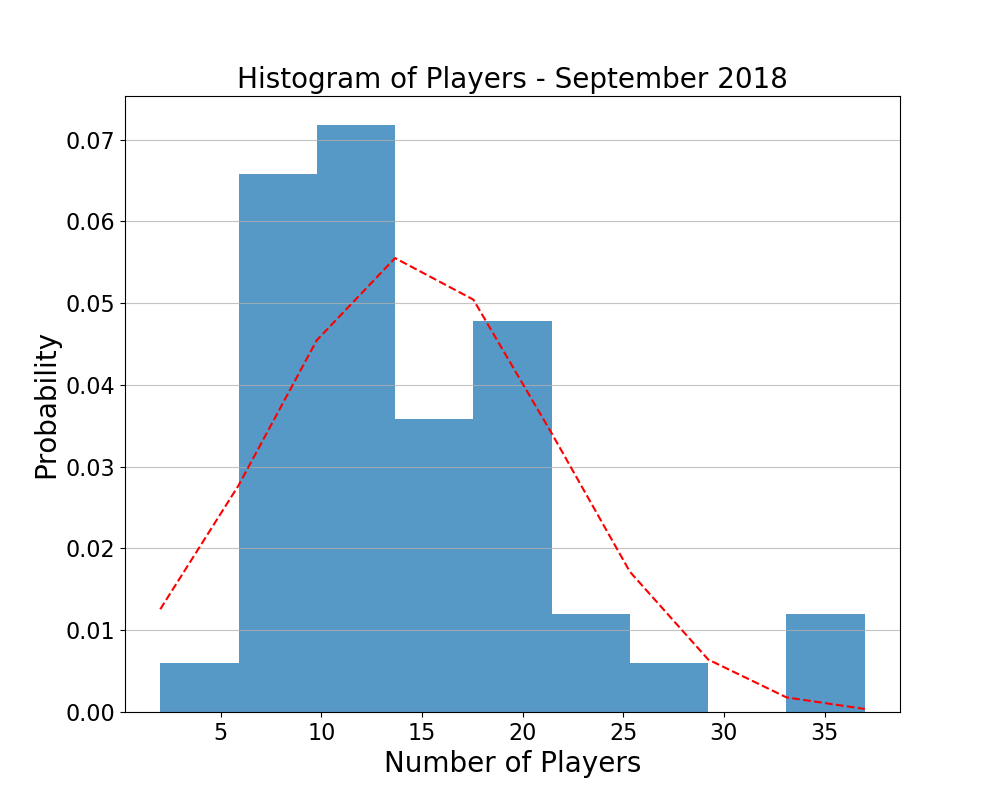
\includegraphics[width=\columnwidth]{../figs/Figure_1.png}
\caption{Histogram of the random variable - number of players. The red dotted line represents the estimation of the random variable's probability.}
\label{fig1}
\end{figure}

Figure \ref{fig1} shows the histogram of the number of players that attended PCs in September. This histogram has been normalized such that the $y$-axis is probability instead of number of occurrences. From this plot we can easily see that the majority of PCs have 8-13 players, events with 13-20 players are less frequent, and events that have 21 or more players are rare. The red line represents a continuous approximation of the probability of having a certain number of players. It essentially confirms that it is more likely to have fewer number of players (8-13) than more players. This is no surprise as this approximation is derived from the histogram.

\section*{September PC Spatial Statistics}

Spatial data is difficult to work with, and even more so when that data is sparse, spread over the entirety of the US, and contains a few clusters of events. This leads to many regions without data to control any analysis (i.e. Montana and Louisiana), and clusters of data that dominate the analysis too much (i.e. Ohio). It's not unlike tightening a screw - too tight and you will strip the screw, making it impossible to undo (clustered data), too loose and the screw will fall out (not enough or sparse data). Ideally we'd want some happy middle ground where the entire US is sampled with events we can collect data from for our analysis. This is impractical for a number of reasons, so instead we do the best with the data we have available, and use that data to better inform where we want data in the future. 

\begin{figure}[ht]
	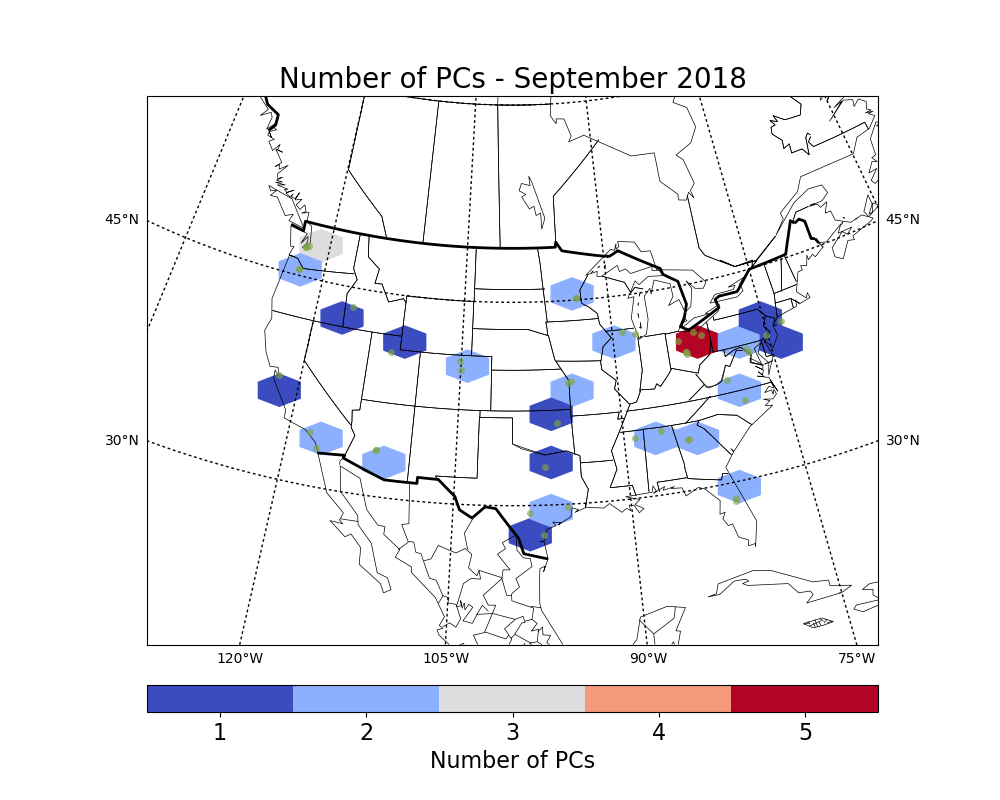
\includegraphics[width=\columnwidth]{../figs/Figure_2.png}
	\caption{Spatial histogram of the number of PCs. Green dots are location where PCs occurred in September.}
	\label{fig2}
\end{figure}

The first spatial metric we will explore is the location of where PCs occurred in September 2018. Figure \ref{fig2} shows a spatial histogram of binned PCs. Each hexagonal bin is approximately 150 miles in diameter. The color is representative of the number of PCs that occur in the same 150 mile diameter bin. The green dots represent the physical location (City and State) of each PC. The first thing we notice is the Ohio ran 5 PCs in September. The next closest is the Seattle area, which ran 3 PCs (5 if the bins supported grouping the 2 PCs in OR). Everywhere else has approximately 1-2 PCs within 150 miles of each other. We also notice that there are large swatches of the country which are uncovered by PCs. This includes New Mexico, Nevada, Montana, Nebraska, the Dakotas, Kentucky, Arkansas, and the far North East. This means that if TOs are to pull in players, those players likely have to drive significant distances to attend events. 

\begin{figure}[ht]
	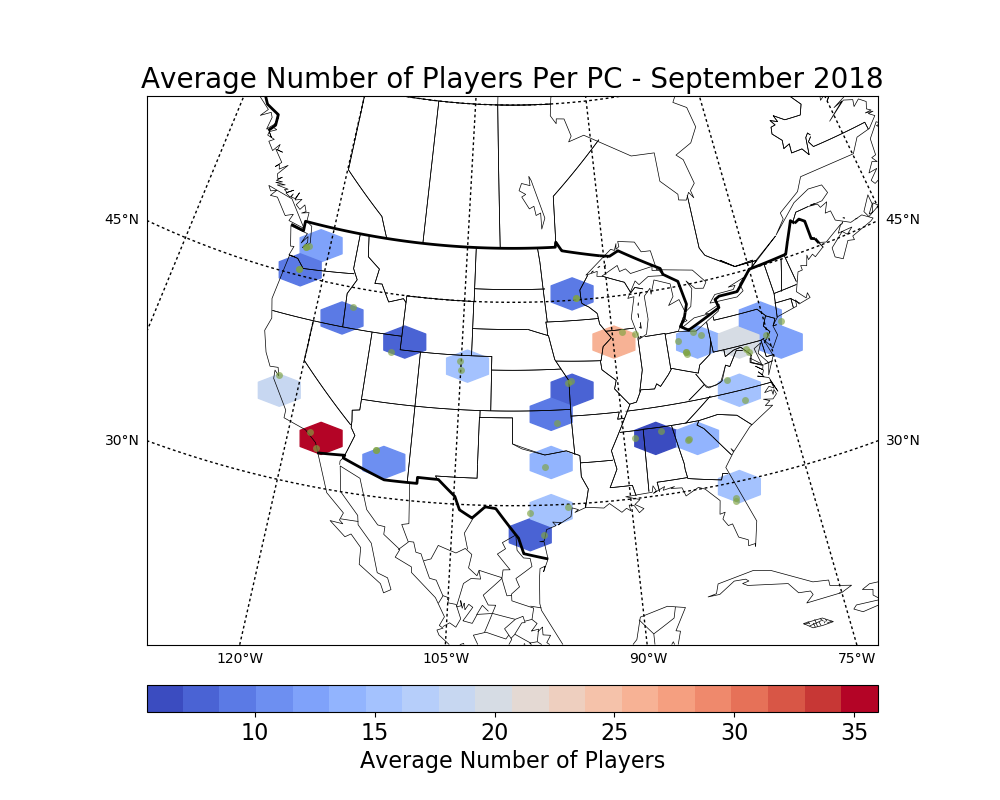
\includegraphics[width=\columnwidth]{../figs/Figure_3.png}
	\caption{Spatial histogram of the average number of players per PC. Green dots are location where PCs occurred in September.}
	\label{fig3}
\end{figure}

If we instead look at the average number of players per PC in each hexagonal bin (total number of players at events in the hexagon divided by the number of events in that hexagon) we see a slightly different story. Instead of seeing Seattle and Ohio as having a large number of players per event, we see that Southern California and Illinois had the most players consistently over the month. Now this isn't news to any TO or player reading this report. Ohio has long been the subject of jokes about being "free CP" (high number of events but only an average number of players), but it's interesting to see in the data regardless. 

\begin{figure}[ht]
	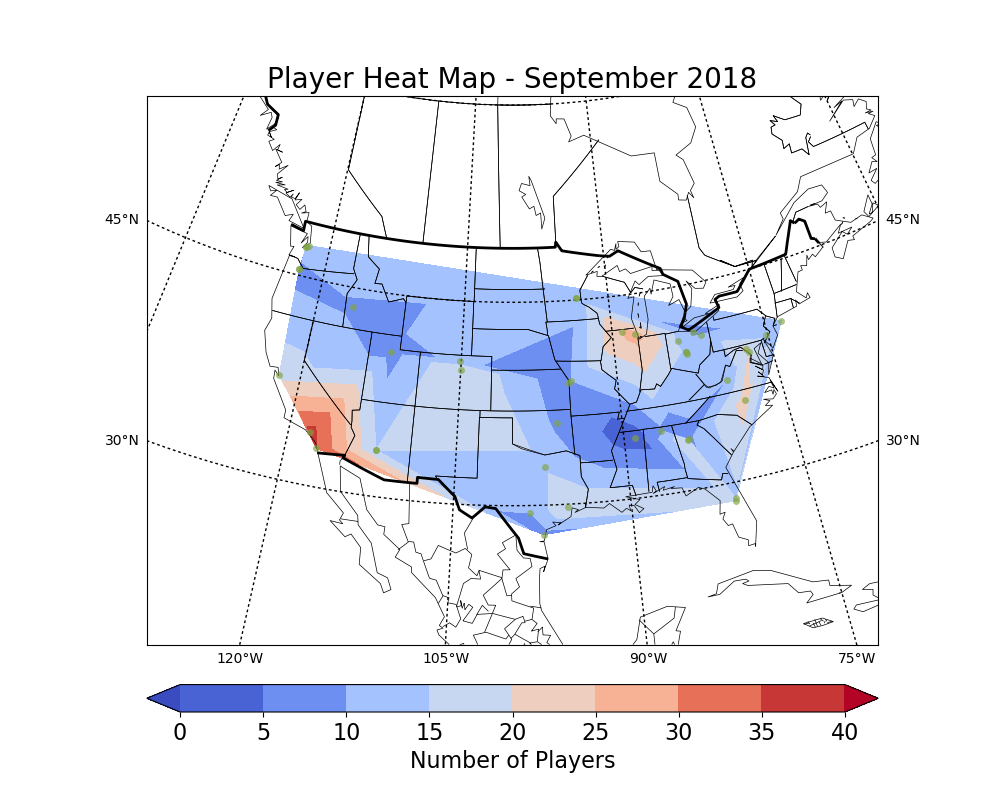
\includegraphics[width=\columnwidth]{../figs/Figure_4.png}
	\caption{Spatial heatmap of the number of players. Green dots are location where PCs occurred in September and are the control points for interpolation.}
	\label{fig4}
\end{figure}

Our final figure for this month is a heat map of players. This map, shown in Figure \ref{fig4}, gives a rough idea of how where players exist across the continuous US. It's quite crude due to the sparsity of the spatial data, but it does highlight additional features in the data. One is the high in the North Carolina and Virginia area on the East Coast, which is a trend that was hidden by the hexagonal binning of the data.

\section*{Discussion and Conclusion}

Personally, I did not find anything too surprising in this month's data. The PCs were about where I expected them, but I expected there to be far more of them. It makes sense that TPCi is in the process of adding more authorized TOs that can help bring VGC to the blank spaces on the maps above. 

The number of players did catch me off guard, as I expected more to show up for the new format. With 617 player registrations this month, with most players having local access to 2 PCs, we can make a ballpark calculation that there were about 300 VGC players in the continuous US this month. That seems small to me because it is roughly the size of the Worlds 2018 Nashville Open, or about 100 players more than the best attended Regional of the last circuit. It especially feels small when the first weekend of the month I judged a local PC that hosted 20 players in Colorado. I had hoped that other TOs had experienced similar increase in attendance, but it seems it was not the case across the board. I hope next month with the return of MSS we see a greater increase in the number of players.

\section*{Future Work}

This month was about laying the framework for what is to come in future months. It is fairly rudimentary analysis with the potential to grow in complexity. In October, MSS make a return to the circuit, and their data becomes relevant once again. Memphis and Portland Regionals will also occur, and have PC and MSS side events as well. The attendance at these Regionals will also start to paint the picture with the September Regionals data. With another month of data, trends can start to be analyzed and questions about player habits and mobility can be answered. 

Mexico and Canada will be included in the October data, with plans to potentially expand to include all of Latin America (making a true North American Report). This should add some needed constraints to the spatial interpolation. TOs that can host PCs, an MSS, are currently being added by TPCi, so we should see data from more locations in the near future to help with spatial constraints. 

As always, if you have any suggestions of what analysis would be beneficial to include, or if you want to lend your help, feel free to reach out on Twitter \href{https://twitter.com/clearcreekVG}{@clearcreekVG} (Colton) or \href{https://twitter.com/PokenomicsDMV}{@PokenomicsDMV} (Kyle), or any other means you have of contacting us. The source code to make the above plots and compile this report is avaliable on \href{https://github.com/ckohnke/pkmheatmap}{Github}.

\section*{Acknowledgments}

The authors would like to thank Kyle Littleton for taking the initiative to aggregate all of the VGC tournament data that is located at the Google Drive Sheet - \href{https://docs.google.com/spreadsheets/d/1ma2g3MTRTx3fUCun9awvshfAFoD9gRbB7rpf7qXve-k/edit?usp=sharing}{2018-2019 US VG Event Info Sheet}. Stephen Cuttler (VGC TO: Colorado School of Mines) also deserves recognition for lengthy discussions on how to best present this data for public consumption.

\end{document}
